% CS6140 Homework Assignment Template
% Computer Science
% Northeastern University
% Boston, MA 02115

% Do not manipulate any of the settings
\documentclass[twoside]{article}

\usepackage{epsfig}
\usepackage{natbib}
\usepackage{units}
\usepackage{amssymb}
\usepackage{amsmath}
\usepackage{babel}
\usepackage{forest}


\setlength{\oddsidemargin}{0 in}
\setlength{\evensidemargin}{0 in}
\setlength{\topmargin}{-0.6 in}
\setlength{\textwidth}{6.5 in}
\setlength{\textheight}{8.5 in}
\setlength{\headsep}{0.75 in}
\setlength{\parindent}{0 in}
\setlength{\parskip}{0.1 in}

\newcommand{\lecture}[3]{
   \pagestyle{myheadings}
   \thispagestyle{plain}
   \newpage
   \setcounter{page}{1}
   \noindent
   \begin{center}
   \framebox{
      \vbox{\vspace{2mm}
    \hbox to 6.28in { {\bf CS6140: Machine Learning\hfill} }
       \vspace{6mm}
       \hbox to 6.28in { {\Large \hfill #1  \hfill} }
       \vspace{6mm}
       \hbox to 6.28in { {\it Assigned: #2 \hfill Due: #3} }
      \vspace{2mm}}
   }
   \end{center}
   \markboth{#1}{#1}
   \vspace*{4mm}
}

\begin{document}

% to have alphanumeric enumeration (Hasan's command)
\renewcommand{\labelenumi}{\alph{enumi})}

\lecture{Homework Assignment \# 4}{03/21/2020}{03/31/2020, 11:59pm, through Blackboard}

\begin{center}
Piyush Goel\\
Email: goel.pi@northeastern.edu
\end{center}

%%
%% Problem
%%

\textbf{Problem 1.} (20 points) Consider a logistic regression problem with its initial solution obtained through the OLS regression; i.e., $\mathbf{w}^{(0)}=(\mathbf{X}^{T}\mathbf{X})^{-1}\mathbf{X}^{T}\mathbf{y}$
, in the context of the code provided in class (Week 6). Recall that $\mathbf{x}$ was drawn from a mixture of two Gaussian distributions with dim$\left\{ \mathbf{x}\right\}=2$ (before adding a column of ones) and that $y \in \left\{ 0, 1\right\}$. You probably noticed that the initial separation line is consistently closer to the data points of class 0.

\begin{enumerate}
\item (10 points) Why was this the case? Draw a picture (if possible) to support your argument.
\item (5 points) Devise a better initial solution by modifying the standard formula $\mathbf{w}^{(0)}=(\mathbf{X}^{T}\mathbf{X})^{-1}\mathbf{X}^{T}\mathbf{y}$.
\item (5 points) Now again consider the case where $y \in \left\{ -1, +1\right\}$. What is the form of the
modified solution from part (b) in this case?
\end{enumerate}

\textbf{Solution}

\begin{enumerate}
	\item
	The formula we use to initialize the weights is the same as the solution of OLS Linear Regression. If we consider this as a linear regression problem instead of a logistic regression one then we have two features (which is the same as in the case of logistic regression), and one output (but the output here is continuous variable, albeit the correct values are binary). So linear regression would look for a 3-D plane with the 3 axes as $X_1, X_2, Y$.\\
	For all the points of class 0 the intersection of the planes $Y=0$ and the plane which is the solution of linear regression would be a line closer to the data points of class 0, since that is how linear regression is supposed to work (i.e. predict a value as close to zero as possible for all the points with $y=0$). Similarly there would be a line closer to the points of class 1 in the plane $Y=1$ as well.\\
	Now, for logistic regression we're only working in two dimensions with axes $X_1, X_2$ or simply the plane $Y=0$, if we try to relate to the linear regression scenario. Hence we only see the intersection of the plane $Y = 0$ and the plane which is the solution of OLS regression, which is line close to the points of class 0.
	
	\item
	Firstly, for simplicity lets assume the number of points of both the classes is roughly the same. For a better initial solution we somehow need to find the line which is the intersection of the OLS regression solution plane and the plane $Y=0.5$ (instead of $Y=0$), since that line should equally be closer to the points of both classes 0 and 1. Or instead of finding the line that we can just shift the whole solution plane down along the Y-axis by 0.5, which can simply be done by adding -0.5 to $w_0$. Therefore a better starting solution would be $\mathbf{w}^{(0)}=(\mathbf{X}^{T}\mathbf{X})^{-1}\mathbf{X}^{T}\mathbf{y} + \begin{bmatrix}
	-0.5\\0\\0
	\end{bmatrix}$.\\
	This was assuming that both the classes have roughly the same number of points. Otherwise instead of the plane $Y=0.5$ a better choice would be $Y = \frac{n_1}{n_0+n_1}$, where $n_0$ and $n_1$ are the number of points belonging to the class 0 and 1 respectively. Therefore a better starting solution would be $\mathbf{w}^{(0)}=(\mathbf{X}^{T}\mathbf{X})^{-1}\mathbf{X}^{T}\mathbf{y} + \begin{bmatrix}-\frac{n_1}{n_0+n_1}\\0\\0\end{bmatrix}$. To help imagine this let $n_0=1000$ and $n_1 = 10$, in this case the solution plane would relatively have a small angle of intersection with the plane $Y=0$ as compared to the case when $n_0 \approx n_1$, hence we only need to shift the plane by a small amount to get a better initialization and shifting by 0.5 might make the line move too far. This might not still be the best initialization, but is certainly better than the simple OLS regression one.
	
	\item
	In this case we don't need to modify our solution since the line which is at the intersection of $Y=0$ and the solution plane would be already be equally close to points of both classes +1 and -1, since 0 is in the middle of +1 and -1. Hence the solution remains $\mathbf{w}^{(0)}=(\mathbf{X}^{T}\mathbf{X})^{-1}\mathbf{X}^{T}\mathbf{y}$.\\
	Again, similar to previous part for the case when $n_0$ and $n_1$ have large difference a better solution would be $\mathbf{w}^{(0)}=(\mathbf{X}^{T}\mathbf{X})^{-1}\mathbf{X}^{T}\mathbf{y} + \begin{bmatrix}0.5-\frac{n_1}{n_0+n_1}\\0\\0\end{bmatrix}$.
	
	
\end{enumerate}



\vspace{1em}
\newpage
%%
%% Problem
%%

\textbf{Problem 2.} (15 points) Let $A$, $B$, $C$, and $D$ be binary input variables (features). Give decision trees to represent the following Boolean functions:

\begin{enumerate}
\item (3 points) $A\wedge\bar{B}$
\item (3 points) $A\vee(B\wedge\bar{C})$
\item (3 points) $\bar{A}\oplus B$
\item (3 points) $(A\wedge B)\vee(C\wedge D)$
\item (3 points) $(A\vee B)\wedge((C\vee\bar{D})\oplus B)$
\end{enumerate}
where $\bar{A}$ is the negation of $A$ and $\oplus$ is an exclusive OR operation.


\textbf{Solution}\\
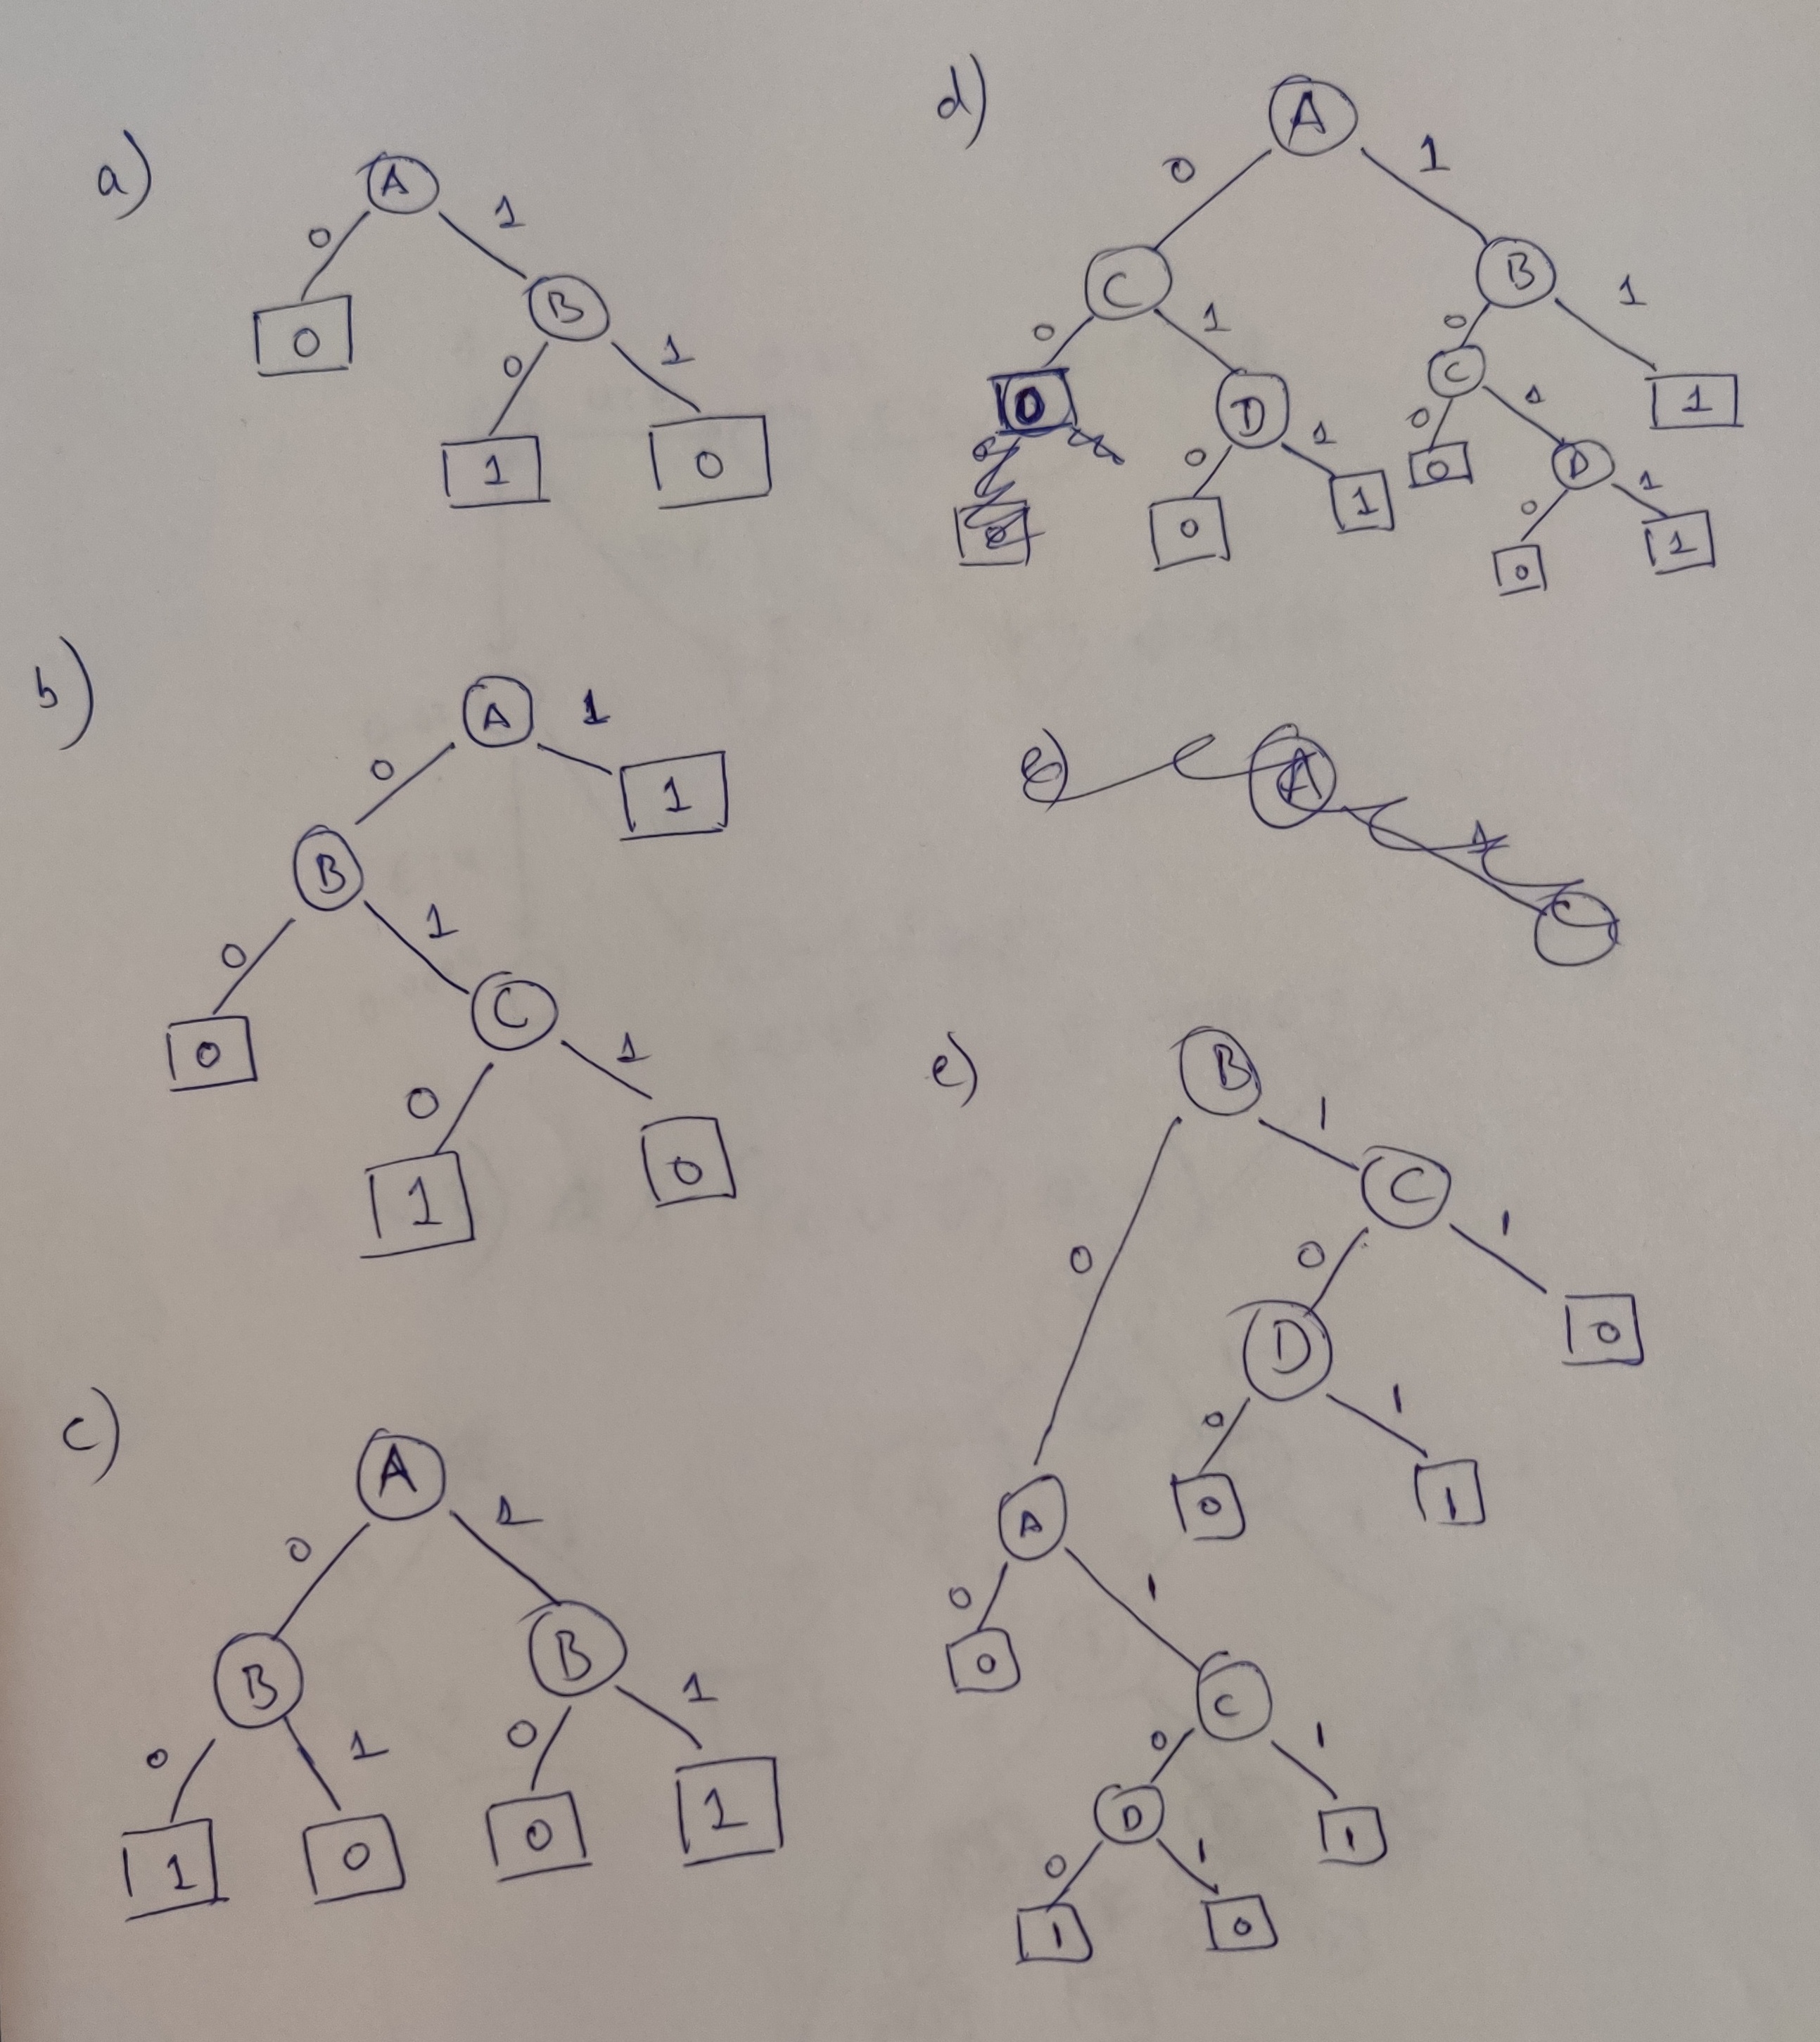
\includegraphics[scale=0.15]{img}



\vspace{1em}

%%
%% Problem
%%

\textbf{Problem 3.} (10 points) Consider the data set from the following table:

\begin{tabular}{|c|c|c|c|c|c|c|c|}
\hline 
 & Sky & Temperature & Humidity & Wind & Water & Forecast & Enjoy Sport\tabularnewline
\hline 
\hline 
1 & Sunny & Warm & Normal & Strong & Warm & Same & Yes\tabularnewline
\hline 
2 & Sunny & Warm & High & Strong & Warm & Same & Yes\tabularnewline
\hline 
3 & Rainy & Cold & High & Strong & Warm & Change & No\tabularnewline
\hline 
4 & Sunny & Warm & Hign & Strong & Cool & Change & Yes\tabularnewline
\hline 
\end{tabular}

\begin{enumerate}
\item (5 points) Using Enjoy Sport as the target, show the decision tree that would be learned if the splitting criterion was information gain.
\item (5 points) Add the training example from the table below and compute the new decision tree. This time, show the value of the information gain for each candidate attribute at each step in growing the tree.
\end{enumerate}

\begin{tabular}{|c|c|c|c|c|c|c|c|}
\hline 
 & Sky & Temperature & Humidity & Wind & Water & Forecast & Enjoy Sport\tabularnewline
\hline 
\hline 
1 & Sunny & Warm & Normal & Weak & Warm & Same & No\tabularnewline
\hline 
\end{tabular}

\vspace{1em}

\textbf{Solution}
\begin{enumerate}
	\item 
	
	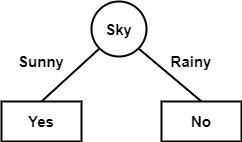
\includegraphics[scale=0.5]{3a.png}
	
	\item
	
	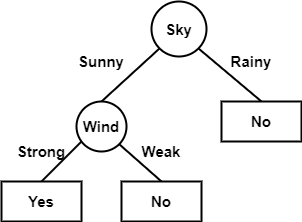
\includegraphics[scale=0.5]{3b.png}
	Information Gain calculation at step 1:\\
\end{enumerate}

%%
%% Problem
%%
\newpage
\textbf{Problem 4.} (40 points) Principal Component Analysis (PCA) as part of dimensionality reduction. Implement PCA yourself with the only allowed library function being the eigenvalue/eigenvector determination. Download at least 3 data sets from the UCI Machine Learning repository (or elsewhere) and learn a logistic regression model in the following three modes:

\begin{enumerate}
\item (5 points) Use the data set as is; i.e., no normalization or any form of preprocessing.
\item (10 points) Normalize the data set using z-score normalization and evaluate the model.
\item (20 points) Normalize the data set to zero mean, apply PCA with 99\% of retained variance, and then train and evaluate the model.
\item (5 points) Normalize the data set using z-score normalization, apply PCA with 99\% of retained variance, and then train and evaluate the model.
\end{enumerate}
In each case, evaluate the model using 10-fold cross-validation. Make sure that all preprocessing steps are performed on training partition only and then applied to the test partition. Provide area under the ROC curve for each model on each data set. To do that, you can average ROC curves obtained on each partition. Discuss your results and provide appropriate support for your conclusions.

\vspace{1em}

\textbf{Solution}

\textbf{No normalization and pre-processing}\\
Dataset: banknote authentication: Avg AUC = 0.99886\\

Dataset: spambase: Avg AUC = 0.9653\\

Dataset: adults with over 50k salary: Avg AUC = 0.80541\\


\textbf{z-score normalization}\\
Dataset: banknote authentication: Avg AUC = 0.99906\\

Dataset: spambase: Avg AUC = 0.96942\\

Dataset: adults with over 50k salary: Avg AUC = 0.83455\\


\textbf{PCA with zero mean normalization}\\
Number of chosen Columns =  4 Total number of Columns =  4\\
Dataset: banknote authentication: Avg AUC = 0.99906\\

Number of chosen Columns =  2 Total number of Columns =  57\\
Dataset: spambase: Avg AUC = 0.75886\\

Number of chosen Columns =  1 Total number of Columns =  14\\
Dataset: adults with over 50k salary: Avg AUC = 0.51027\\


\textbf{PCA with z-score normalization}\\
Number of chosen Columns =  4 Total number of Columns =  4\\
Dataset: banknote authentication: Avg AUC = 0.99931\\

Number of chosen Columns =  54 Total number of Columns =  57\\
Dataset: spambase: Avg AUC = 0.96903\\

Number of chosen Columns =  14 Total number of Columns =  14\\
Dataset: adults with over 50k salary: Avg AUC = 0.83534\\
	
	
Now, as we can see the average AUC-ROC (which is indicative of accuracy) for almost all of the datasets increase from part a to b then decreases for part c and then again increases for d. Therefore the final order is $b > a > d > c$. This can be explained as follows:\\
$b>a$: because we just normalize the data in part b over part a and this may help the learning process, but not too much, hence the increase is almost insignificant. \\
$c < a, c < b, d < b, d < c$: because we're doing PCA which removes some amount of information by removing the features with low variance contribution to the data.\\
$d > c$: Since, during z-score normalization we divide each feature value by the feature's standard-deviation as well and not just subtract the mean, this helps scale down the feature values, effectively lowering the variance of the feature as well. This results in a higher (much higher in some cases) number of features being selected in when PCA is done after z-score normalization instead of zero mean normalization. Hence the better results for part c.


%%
%% Problem
%%

\textbf{Extra Problem.} (25 points) Consider a data set $\mathbf{X}\in\mathbb{R}^{n\times d}$ such that $d\gg n$. Propose how to perform principal component analysis if one must avoid the construction of a large $d\times d$ covariance matrix. You can assume that a $d \times n$ matrix can fit in the memory. This is an all or nothing question. If your result is correct you get 25 points; if not, you get 0 points.


\end{document}
